%%=============================================================================
%% Methodologie
%%=============================================================================

\chapter{WebAR-Article}
\label{ch:webar-article}

%% TODO: Hoe ben je te werk gegaan? Verdeel je onderzoek in grote fasen, en
%% licht in elke fase toe welke stappen je gevolgd hebt. Verantwoord waarom je
%% op deze manier te werk gegaan bent. Je moet kunnen aantonen dat je de best
%% mogelijke manier toegepast hebt om een antwoord te vinden op de
%% onderzoeksvraag.

Dit hoofdstuk bespreekt de eerste poging van het onderzoek dat uitgevoerd werd. Er werd gestart vanuit het downloadbaar project van Google: WebAR-Article. Dit proiect bevat al bijna alle functies die wij willen bereiken in dit onderzoek namelijk: het plaatsen van een 3D-object met AR, Het verplaatsen van het object nadat het geplaatst is, het draaien van het object, een indicator die aanduidt hoe en waar het object in de omgeving zal geplaatst worden en nog enkele functionaliteiten. 
Na het installeren van het project werd er onderzocht naar hoe het tonen van het object kon aangepast worden naar de wens van dit onderzoek. Rekening houdend met dat er in deze bachelorproef gefocust wordt op webshop functionaliteiten werden dan de volgende doelstellingen opgesteld: 

\begin{enumerate}
	\item Astronaut model veranderen: het moet mogelijk zijn het astronaut-model te wijzigen in een ander object naar keuze. Een mogelijk product.
	\item Eigen interactie toevoegen: het moet mogelijk zijn om indien er op het object getikt wordt, er een 2de object in de wereld verschijnt en indien daarop getikt wordt. er doorverwezen wordt naar de winkelmand pagina met dat specifieke product erin.  
	\item Linken aan bestaande webshop? 

\end{enumerate}

\section{Het project}
\label{sec:het-project}

WebAR-Article is een project gecreëerd door Reza Ali, een digitale designer en programmeur die zich bezig houdt met software voor grafisch en dynamisch design, computergegenereerde meetkunde, design tools enzovoort. Reza Ali heeft dit project in functie van Google gedesignd, geïmplementeerd en open source gezet voor andere ontwikkelaars. Het project bevat de licensie Apache License Version 2.0, wat ons toelaat dit te aan te passen en te verspreiden op voorwaarde dat Google zijn copyrightvermeldingen behoudt en dat er een Apache License wordt meegeleverd. 

Zoals vermelde in sectie \ref{sec:state-of-the-multinationals} State of the art, is dit project een simpele pagina die wat weg heeft van Wikipedia. Het bevat één enkele overzichtspagina met wat informatie over de astronaut. Enkele links die naar niets verwijzen maar die dus dienen ter illustratie. In de overzichtspagina van de astronaut is een kader waarin het astronautenobject zichtbaar is. Indien u als gebruiker vanop een computer naar deze website surft kun u de astronaut bekijken in een fictieve wereld. Dit werd waarschijnlijk zo geïmplementeerd aangezien de meeste computercamera's niet voldoen aan de vereisten voor AR te tonen. Om te kunnen genieten van dit project en de astronaut te kunnen plaatsen in uw omgeving met een tablet of smartphone zijn er eerst enkele stappen die uitgevoerd moeten worden. Het project moet namelijk van op een computer met behulp van node en node package manager opgestart worden als server. Vervolgens moet ook de tablet of smartphone de juiste app hebben staan. Dit is omdat de mobiele browsers van op dit moment zoals Google Chrome en Safari nog geen AR ondersteunen. Afhankelijk van of het apparaat een iOS of Android besturingssysteem draait, moet het de app WebARonARKit of WebARonARCore hebben. In dit onderzoek werd er getest met een iPhone 6s met WebARonARKit.

\begin{figure}
	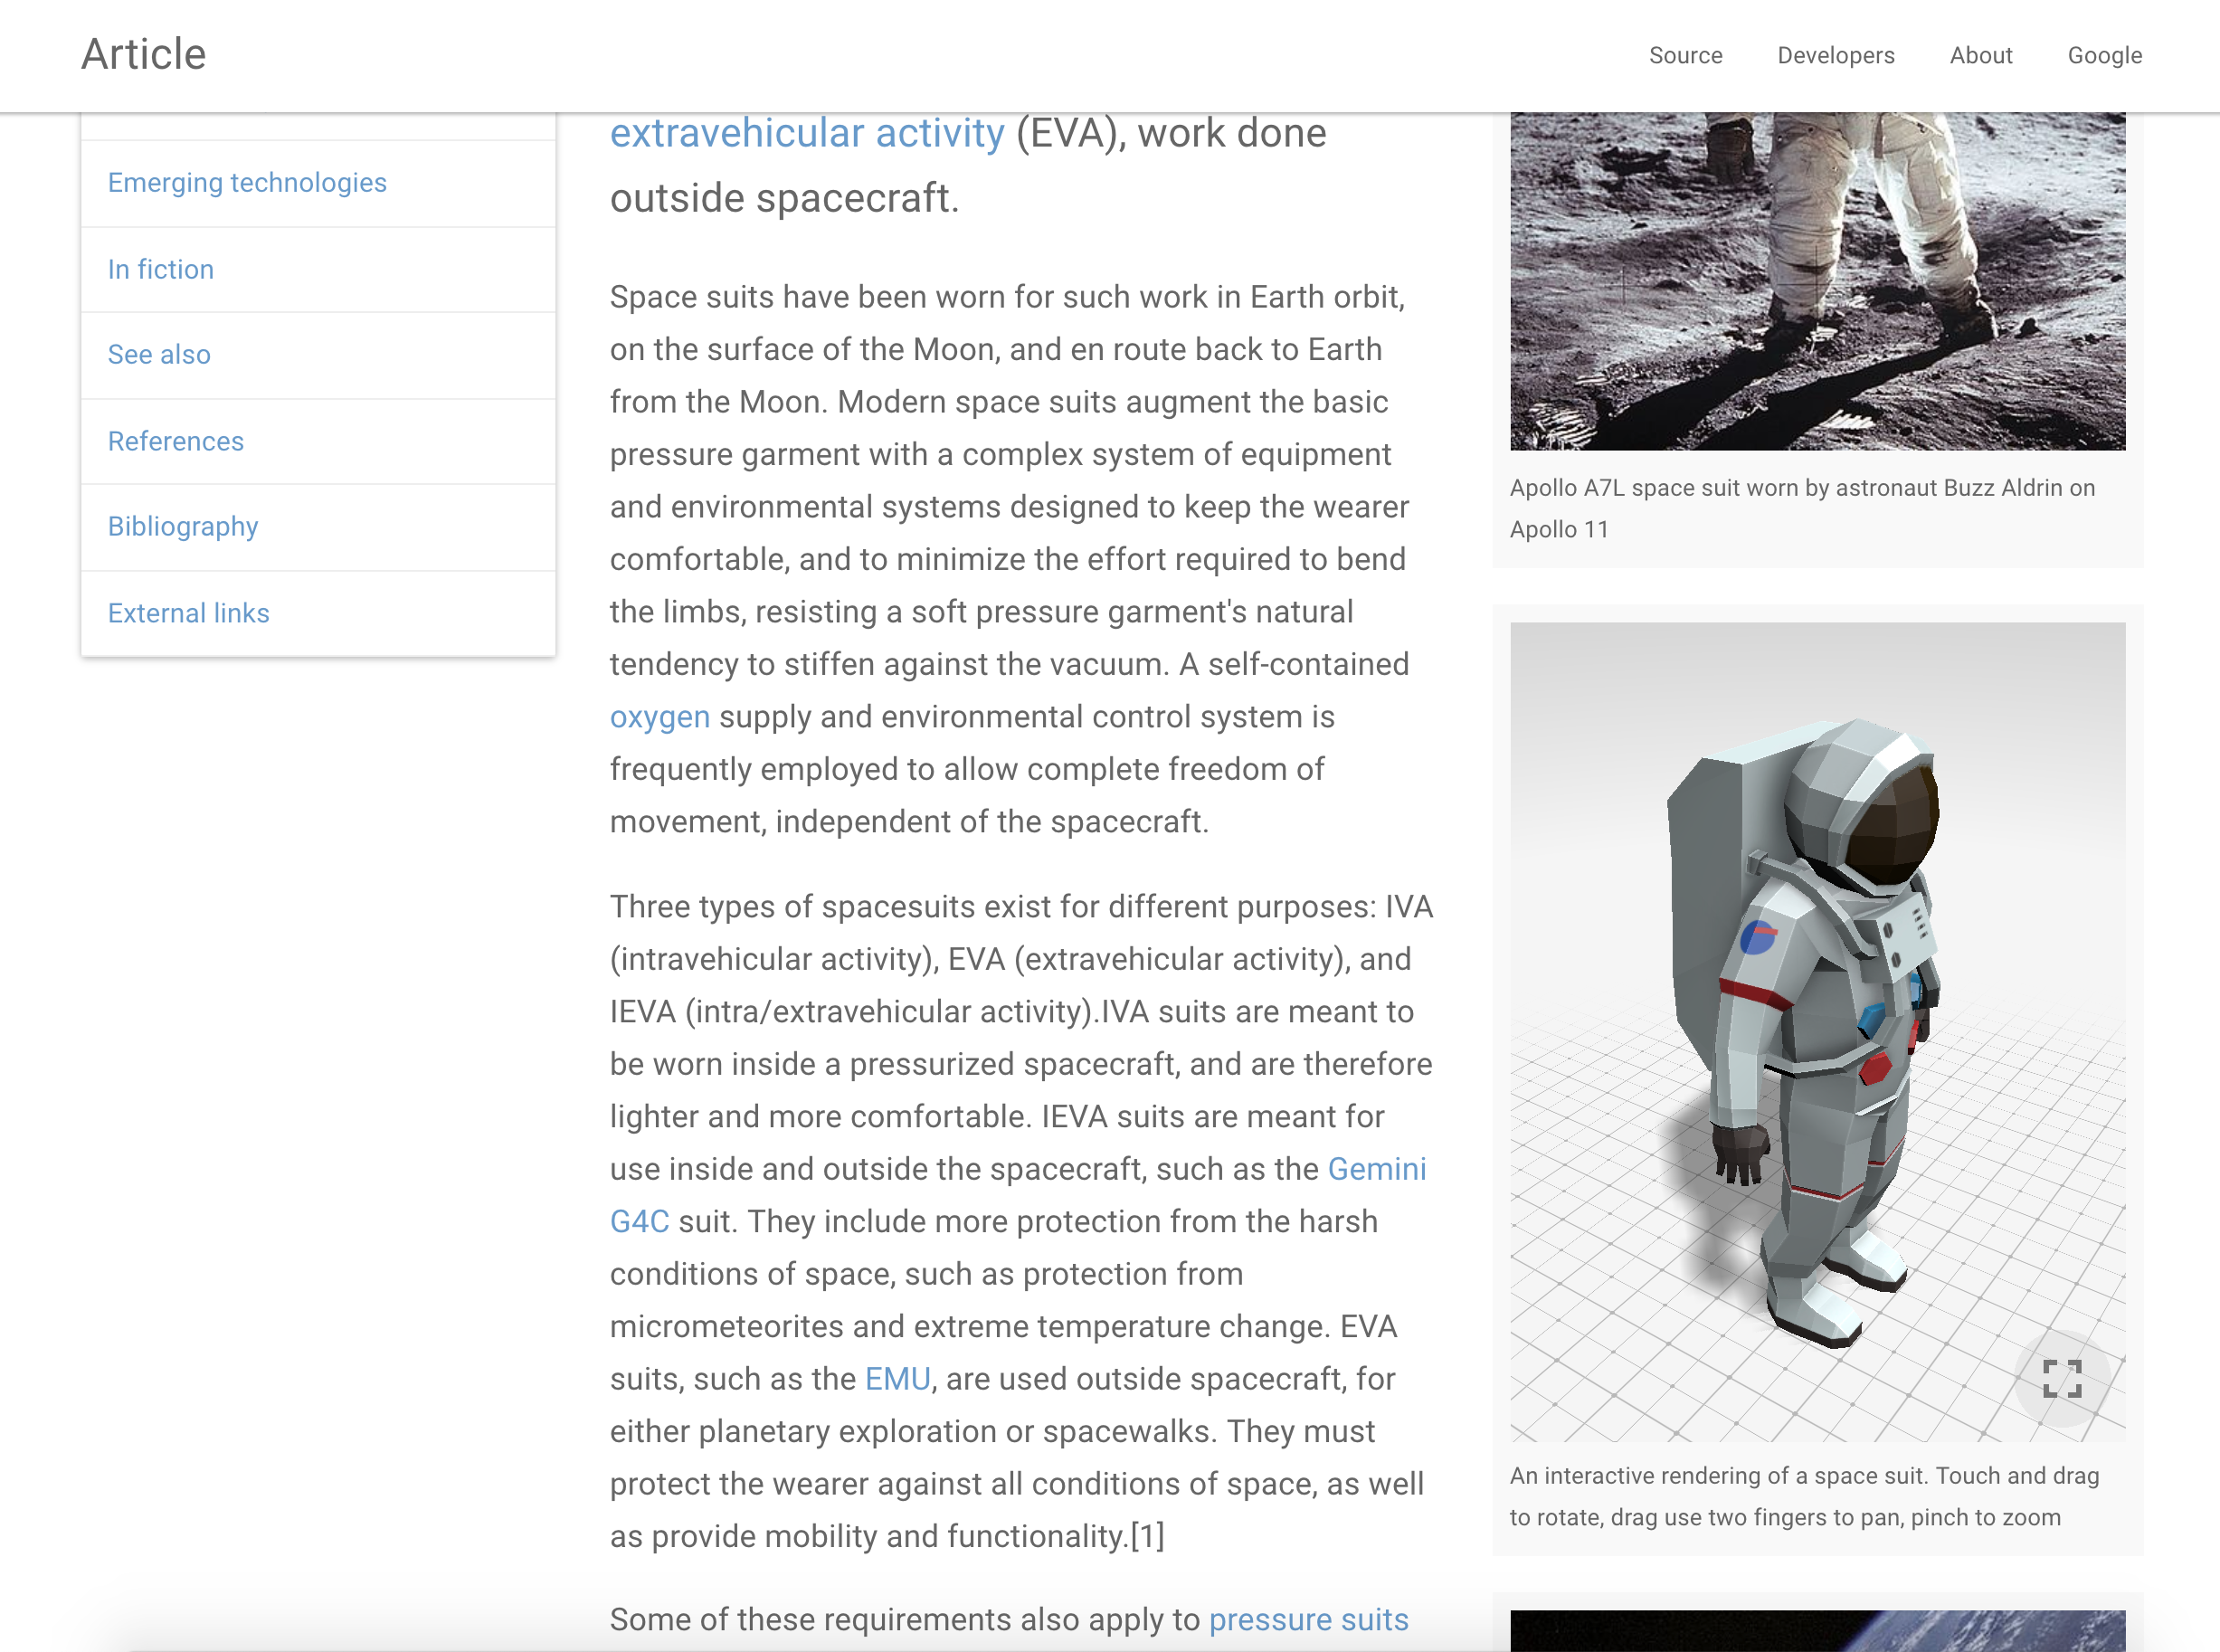
\includegraphics[width=\linewidth]{img/WebARArticle.png}
	\caption{Het project wanneer bekeken op een computer \autocite{Ali2018}.}
\end{figure}

\section{WebARonARKit}
\label{sec:WebARonARKit}

WebARonARKit is een niet-officiële app die op ironisch wijze gemaakt is geweest door Google. Als u de app opent ziet u een soort van minimalistische browser, dit omdat het niet bedoeld was als volledig uitgeruste webbrowser, waarmee u AR ervaringen mee kan beleven. Om de app te downloaden kunt u terecht op de repository van ~\textcite{Google2018}. Hierop staan er ook links naar testbare voorbeelden en staat er in detail uitgelegd hoe u de app op uw smartphone kan krijgen. 

\textbf{Structuur}

WebARonARKit bestaat uit 2 primaire onderdelen namelijk een instantie van WKWebView en de extensies voor de WebVR API. 

Apple heeft voor ontwikkelaars een klasse oftewel een soort van onderdeel met zijn eigen functionaliteit geschreven, genaamd WKWebView. Het laat ontwikkelaars toe om web vensters in te sluiten in de apps die ze programmeren en op die manier kan de hardware van het apparaat gecombineerd worden met webpagina's via speciale API's. 
Verder maakt WebARonARKit gebruik van uitbreidingen op de nu verouderde WebVR API. Aangezien er bij VR sprake is van een volledig fictieve wereld werden de extra aspecten zoals motion tracking, tonen van de camera en environmental understanding geïmplementeerd in de app. 

\textbf{Werking}

Op het moment dat de webpagina geladen is in de WKWebView, wordt er een script uitgevoerd genaamd WebARonARKit.js. Dit zorgt voor een vlotte en verstaanbare data flow tussen de website en de sensoren van het apparaat. 

Terwijl WebARonARKit in een AR-simulatie zit wordt de camera van het toestel getoond met daar bovenop een doorzichtig webvenster. De synergie hiervan creëert een vlot resultaat tussen wat men door de camera ziet en wat er gevisualiseerd wordt op het scherm. 

\section{Het model veranderen}
\label{sec:het-model-veranderen}

De eerste cruciale stap en misschien wel de meest voldoening gevende stap van dit project is het model veranderen. Want wat ben je met een coole AR functionaliteit op je website als je maar 1 object kan tonen?

%Op het web zijn er verscheidene 3D objecten te vinden uit verschillende bestandsformaten. Zo haalt ~\textcite{Chakravorty2019} aan dat 

Bij het onderzoeken hoe het laden en tonen van het gebuikte model ineen zit viel er iets merkwaardigs op. Het bestandsformaat van het astronautenmodel die gebruikt werd in het project was verschillend van het astronautenmodel in de beschrijving van het project. In de beschrijving wordt er verwezen naar een astronautenmodel te vinden op poly.google.com, een platform waar gebruikers 3D-creaties kunnen op delen en beoordelen. Het astronautenmodel uit het project heeft echter een ander bestandsformaat namelijk .drc. wat staat voor Draco.

\subsection{Draco}

Draco is een open-source bibliotheek gemaakt door het Chrome Media team  die dient voor het decoderen en encoderen van 3D polygon mesh\footnote{Polygon mesh: een polygon mesh is een verzameling van vlakken, kanten en hoogtepunten die de vorm van een object in 3D bepalen. } data. Applicaties die gebruik maken van Draco om hun 3D-objecten te comprimeren zijn veel kleiner in opslag en dit zonder kwaliteitsverlies. Een gevolg daarvan is dat de objecten veel sneller kunnen laden en gebruikers veel minder lang hoeven te wachten om de AR-ervaring te beleven.~\textcite{Nedrich2019} haalt met 2 voorbeelden aan dat modellen die qua grote in de tientallen megabytes liggen, tot ongeveer 5\% van hun oorspronkelijke grote gecomprimeerd kunnen worden. Modellen die slechts enkele megabytes groot zijn, hebben het daar moeilijker mee. 

Om Draco te kunnen gebruiken staat er een handleiding hoe u dit installeert en klaarzet op de repository van dit project. In dit onderzoek werd het eerst geïnstalleerd voor het MacOS specifieke programma XCode. Echter is het gebruik hiervoor niet gedocumenteerd en werd er niet in geslaagd objecten naar .drc te encoderen. Nadien werd Draco zodanig geïnstalleerd dat het encoder en decoderen kon gestart vanuit commando's

\textbf{Het de-en encoderen van het object}

Eenmaal geïnstalleerd is het mogelijk objecten naar .drc te comprimeren met behulp van het commando: \textbf{./draco\_encoder -i bestansnaam.ply -o bestandsnaam.drc} of het commando \textbf{./draco\_encoder -i bestansnaam.obj -o bestandsnaam.drc}. Let hier wel bij op dat opdat dit commando kan slagen, het een object moet krijgen als invoer van het type ply of obj. 

MOET NOG VERTELD WORDEN OVER HET EFFECTIEF DECODEREN EN ENCODEREN VAN ANDERE OBJECTEN. EN DE PROBLEMEN MET MATERIALS ENZO
%Problemen met aangepaste modellen door de materials. Het is onduidelijk hoe dit op te vangen is met draco

\section{Eigen interactie toevoegen}
\label{sec:eigen-interactie-toevoegen}

\section{Linken aan bestaande webshop}
\label{sec:linken-aan-bestaande-webshop}



